%!TEX root = HitchinSystems.tex

\chapter{Geometric Langlands and Mirror Symmetry}

In this chapter we will describe of the following result of
Hausel-Thaddeus \cite[Theorem 3.7]{HT}:
\begin{thm}
Let $X$ be a compact Riemann surface, let $M^d_{SL_n}$ be the Hitchin
moduli of stable $SL_r$-principal bundles of degree $d$ and
$M^e_{PGL_r}$ the analogous moduli for $PGL_r$. Then $M^d_{SL_r}$ and
$M^e_{PGL_r}$ are SYZ-mirror dual.
\end{thm}

Our exposition has essentially three parts: firstly we describe what
we understand by SYZ-mirror symmetry, secondly one describes the above
moduli spaces more explicitly using the Hitchin moduli space for
$GL_r$ we are used to in the class. Finally, we give some elements of
the proof which boils down to a study of the abelian varieties that
appear as fibers of the Hitchin fibration and of universal families
over the Hitchin moduli space for $SL_r$ and $PGL_r$.

\section{Strominger-Yau-Zaslow mirror symmetry proposal}

Let $M$ be a \emph{Calabi-Yau manifold}, i.e. a K\"ahler manifod with
fundamental form $\omega$ and also a (covariant) constant holomorphic
$n$-form $\Omega$, where $n=\mbox{dim}_{\mathbb{C}}(M)$\footnote{Another
  description of a Calabi-Yau is as a manifold $M$ with a triple
  $(\omega,\Omega^r,\Omega^i)$ of a $2$-form and two $n$-forms s.t.
\begin{enumerate}[(i)]
\item $\omega$ is non-degenerate;
\item $\Omega^r + i\Omega^i$ is locally $dz_1\wedge dz_2
  \wedge\cdots\wedge dz_n$ and non-vanishing;
\item $\Omega^r\wedge\omega=\Omega^i\wedge\omega =0$;
\item
  $\left(\Omega^r+i\Omega^i\right)\wedge\left(\Omega^r-i\Omega^i\right)=\omega^n$
(or $i\omega^n$);
\item all three are closed;
\item for all non-zero $v\in \Gamma(M,T_{\mathbb{C}}M),
  \omega_{\mathbb{C}}(v,\bar{v})>0$. 
\end{enumerate}
In particular, if
  $(M,\omega_1,\omega_2,\omega_3)$ is Hyperk\''ahler of complex
  dimension $2m$, then $\Omega^r+i\Omega^i \equiv
  \left(\omega_3+i\omega_1\right)^{\wedge m}$ with $\omega_2$ satisfy
  the above. For details see the nice paper by Hitchin \cite{H4}.}.

Suppose there exist a real $n$-dimensional manifold $N$, and another
Calibi-Yau $\check{M}$ manifold (more generally orbifold) with maps:

\begin{figure}[h!]
\centering
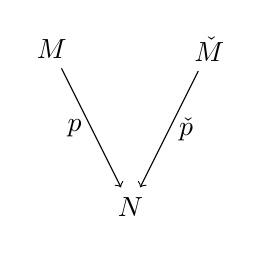
\begin{tikzpicture}
\draw (0,0) node (a) {$M$};
\draw (2,0) node (b) {$\check{M}$};
\draw (1,-2) node (c) {$N$};
\draw [->] (a) --node[left]{$p$} (c);
\draw [->] (b) --node[right]{$\check{p}$} (c);
\end{tikzpicture}
\end{figure}

Then \cite{SYZ} say $M$ and $\c{M}$ are mirror dual if they satisfy:
\begin{enumerate}[(i)]
\item For all regular points $x \in N$, $L_x\equiv p^{-1}(x)$ and
  $\check{L}_x\equiv \check{p}^{-1}(x)$ are \emph{special Lagrangian tori},
  i.e. $L$ is a torus, $\left.\omega\right|_{L}=0$ (Lagrangian) and
  $\left.\mbox{Im}(\Omega)\right|_{L}=0$ (special).
\item $L_x$ and $\check{L}_x$ are dual abelian varieties\footnote{Given
    $A$ an abelian variety over a field $k$, we define the functor
$\sP_A: \mbox{Sch}_{k} \rightarrow \mbox{Set}$ given by:
\[\sP_A(S) = \left\{\mbox{degree 0 line bundles } \sL \mbox{ over }A\times S \; | \;
\left.\sL\right|_{\{1\}\times S} \simeq \sO_S\right\},\]
where $1 \in A$ is the unit. A non-trivial important fact is that
$\sP_A$ is representable, the \emph{dual abelian variety} $\check{A}$ is
the representing object.}. In their formulation one actually requires
a weaker condition: that $L_x$ is a torsors for an abelian variety and
is in bijection with $\check{L}_x$ which is a torsor for the dual abelian
variety.
\end{enumerate}

\begin{rem*}
In general it is hard to produce special Lagrangian tori, however in
the case where $M$ comes from a Hyperk\"ahler manifold as explain in
the footnote any complex (for the $J_2$ structure) Lagrangian is
special. This will be the case for the Hitchin moduli spaces.
\end{rem*}

Before we focus on the example at hand, let's consider a slight
generalization of the above. One reference for this version of mirror
symmetry is also work of Hitchin \cite{H5}. In general
one might not have that the fibers of the above correspondence are
groups, but they might only be torsors for some abelian
variety $A$. Suppose that this abelian variety is $A \simeq
H^1(X,U(1))$ for some $X$, i.e. it is the Picard variety of some
curve. One wants to say that $L_x$ is a torsor for $H^1(X,U(1))$
geometrically. Note that if one has a trivial $U(1)$-bundle $L$ over
$X$, then the space of trivializations of $L$ is a
$H^0(X,U(1))$-torsor. This motivates one to consider a geometric
object over $X$, whose space of trivializations is a
$H^1(X,U(1))$-torsor.

\begin{defn}
Let $BU(1)$ be the sheaf\footnote{More precisely, $\sG$ over $X$ is a
  sheaf of categories (or groupoids) if for all $f: S \rightarrow X$ a cover,
  one has a data $f^*:\sG(X) \rightarrow \sG(S)$, and for $f^{(2)}:S^{(2)} \rightarrow
  S^{(1)}$ one has $\theta_{1,2}:f^{(2),*}\circ f^{(1),*} \rightarrow \left(f^{(1)}\circ
    f^{(2)}\right)^*$ satisfying:
\begin{enumerate}[(i)]
\item (\textit{presheaf}) $\theta_{1,23}\circ\theta_{2,3} = \theta_{12,3}\circ
  \theta_{1,2}$ for any chain of covers $S^{(3)}\overset{f^{(3)}}{\rightarrow}
  S^{(2)}\overset{f^{(2)}}{\rightarrow}S^{(1)}\overset{f^{(1)}}{\rightarrow}S \rightarrow X$;
\item (\textit{sheaf for morphisms}) For $X = \sqcup_{I}S_i$, then
  $g:P_1 \rightarrow P_2$ between two objects of $\sG(X)$ is specified by
  $g_i:\left.P_1\right|_{S_i}\rightarrow \left.P_2\right|_{S_i}$ for all $i$,
  such that $\left. g_i\right|_{S_{ij}} = \left.g_j\right|_{S_{ij}}$;
\item (\textit{sheaf for objects}) For $X = \sqcup_{I}S_i$, $Q_i \in
  \sG(S_i)$, with $u_{ij}:\left.Q_i\right|_{S_{ij}}\simeq
  \left.Q_i\right|_{S_{ij}}$ such that $u_{ij}u_{jk} = u_{ik}$, then
  there exists $Q \in \sG(X)$ glueing these objects.
\end{enumerate}
} of Picard
groupoids\footnote{A \emph{Picard groupoid} just means a groupoid
  which has a symmetric monoidal structure, where all objects are
  invertible, morally a group-object in the category of symmetric
  monoidal categories.} over $X$ given by: for every $U$ an open of
$X$
\[BU(1)(U) = \left\{U(1)\mbox{-torsors over }U\right\}.\]
A $U(1)$-\emph{gerbe} is a sheaf of Picard groupoids $\sA$ over $X$,
s.t. locally $\sA \simeq BU(1)$\footnote{One can continue to spell out
the details: $\sA$ is a gerbe for $A$ (a sheaf of groups on $X$) if it
is a sheaf of categories (we keep the same notation as before) and in
addition one has the conditions:
\begin{enumerate}[a.]
\item For all $i$, $Q_i \in \sA(S_1)$, $\mbox{Aut}(Q_i)$ is an
  $A$-torsor on $S_i$;
\item For all $Q_1,Q_2 \in \sA(S_1)$ there exists $\tilde{S}_1$,
  s.t. $\left.Q_1\right|_{\tilde{S}_1}\simeq
  \left.Q_2\right|_{\tilde{S}_1}$;
\item There exist a cover $\tilde{X} \rightarrow X$,
  s.t. $\sA(\tilde{X}) \neq \empty$.
\end{enumerate}}.
\end{defn}

\begin{rem*}
In the definitions in the footnotes we always think of \'etale
covers. We warn the reader that the notions of sheaf of categories,
groupoids, gerbes, etc. are very sensitive to the topology one uses.
\end{rem*}

We will note torture the reader with the definition of an isomorphism
between gerbes, see \cite{Br,DG} for details. The important take away
from it is the following two properties.

\begin{prop}
The isomorphism classes of $U(1)$-gerbes over $X$ are in bijection with
$H^2(X,U(1))$. Moreover, given $\sB$ a trivial $U(1)$-gerbe over $X$,
the space of trivializations of $\sB$, denoted
$\mbox{Triv}^{U(1)}(X,\sB)$ is a $H^1(X,\sB)$-torsor.
\end{prop}

Finally we reformulate the proposal of mirror symmetry as
follows. Suppose that in addition to the diagram above one also has
the data of $\sB$ a $U(1)$-gerbe over $M$ and $\check{\sB}$ a
$U(1)$-gerbe over $\check{M}$. Then, we say they are mirror dual to
each other if for all $x \in N$ regular:
\begin{enumerate}[(i)]
\item $L_x \simeq
  \mbox{Triv}^{U(1)}(\check{L}_x,\left.\check{\sB}\right|_{\check{L}_x})$;
\item $\check{L}_x \simeq
  \mbox{Triv}^{U(1)}(L_x,\left.\sB\right|_{L_x})$.
\end{enumerate}

\begin{rem*}
Note one needs to require both conditions, which was redundant before
since taking the double dual of an abelian variety is canonically
the identity.
Also, note that promoting the bijection of sets in the original
definition to a bijection of torsors is only a non-trivial statement
when made in families, in other words the use of gerbes is inevitable
in this situation.
This proposal was put forth first in \cite{H5} where he is trying to
make sense of what B-field are, i.e. the extra data of the gerbe
considered here.
\end{rem*}

\section{Hitchin moduli}

Fix a curve $X$ and $x_0 \in X$ a point. Let's recall that
\[M^d_{GL_r} = \left\{\mbox{stable degree d }GL_r-\mbox{principal
    bundles } E
  \mbox{ over }X \; | \; \psi \in H^0(X,\mbox{End}(E)\otimes
  K_X)\right\}\]
We first construct $M^d_{SL_r}$. Consider the map $\det: M^d_{GL_r}
\rightarrow M^d_{\mathbb{C}^{\times}}$ given by
\[\det((E,\psi)) = (\wedge^{r}E, \mbox{tr}\psi),\]
note that one obtains the trace of the Higgs field because one has to
consider the derivative of the determinant as the induced map on the
associated adjoint bundle. Let $(\sO_X(dx_0),0) \in
M^d_{\mathbb{C}^{\times}}$, then define $M^d_{SL_r}$ by the pullback diagram
\begin{figure}[h!]
\centering
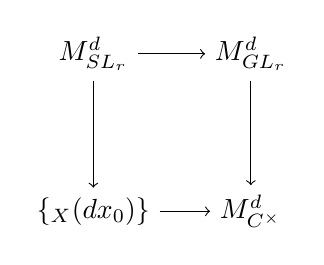
\begin{tikzpicture}
\draw (0,0) node (a) {$M^{d}_{SL_r}$};
\draw (2,0) node (b) {$M^{d}_{GL_r}$};
\draw (0,-2) node (c) {$\{\sO_X(dx_0)\}$};
\draw (2,-2) node (d) {$M^d_{\mathbb{C}^{\times}}$};
\draw [->] (a) -- (b);
\draw [->] (a) -- (c);
\draw [->] (c) -- (d);
\draw [->] (b) -- (d);
\end{tikzpicture}
\end{figure}

More concretely, one has $M^d_{SL_r}=\left\{(E,\psi) \in M^d_{GL_r} \;
  | \; \wedge^rE \simeq \sO_X(dx_0), \mbox{ and tr}(\psi) =
  0\right\}$.

Analogously for $M^d_{PGL_r}$. Recall that
\[1 \rightarrow \mu_r \rightarrow SL_r \rightarrow PGL_r \rightarrow 1\]
is an exact sequence which defines $PGL_r$. Let 
\[ \Gamma^r = \left\{\sL
\mbox{ degree 0 line bundle over }X \; | \; \sL^{\otimes r} =
\sO_X\right\},\] 
i.e. the $r$-torsion point of $\mbox{Pic}^0(X)$. Then
define $M^d_{PGL_r} = M^{d}_{SL_r}/\Gamma^r,$ where $\sL \in \Gamma^r$
acts by $(E,\psi) \mapsto (E\otimes \sL,\psi \otimes \sL)$.

We will denote by $B = \oplus^r_{i \geq 2}H^0(X,K^{\otimes i}_X)$ the
base of both Hitchin moduli, and by $\mu: M^d_{GL_r} \rightarrow B$ and
$\check{\mu}:M^d_{PGL_r} \rightarrow B$ the fibrations obtained by taking the
characteristic polynomials. Note that one does not have the first term
because of the traceless condition.

\begin{rem*}
For the reader that finds our construction of these moduli spaces
ad-hoc we remark that there is a general definition of these moduli
space for all reductive groups due to Simpson. It agrees with the one
took for $SL_r$ and $PGL_r$. The advantage of the one we adopted is
that one does not need to worry about what stability means for a
general principal $G$-bundle, which can be a little subtle.
\end{rem*}

Here is what we will prove in the next section. 
\begin{thm}
For any $(d,e) \in
\bZ\times \bZ$ there exist $U(1)$-gerbes $\sB^e$ over $M^d_{GL_r}$ and
$\check{\sB}^e$ over $M^e_{GL_r}$ such that they are mirror dual in the
generalized sense described in the last section.
\end{thm}

\begin{rem*}
Another prediction of mirror symmetry is a compatibility of the stringy
Hodge numbers. The paper \cite{HT} also has results in this direction
which we will not talk about here.
Note that $SL_r$ and $PGL_r$ are Langlands dual to each other. One can
ask if a similar duality holds in more generality, and that is true
and is the content of \cite{DP}.
\end{rem*}

\section{Universal families}

The title of this subsection is to involke what I believe is the
essential ingredient in the proof of the above result.

Henceforth $B$ will denote a Zariski open of the basis of the Hitchin,
defined by $x \in B$ such that the associated spectral curve
$\Sigma_x$ is smooth.

\textit{Step 1 (indentify the fibers):}
Recall that in $M^d_{GL_r}$ for a fixed
value of $x$, the characteristic polynomial, one has (cf. Lei's first
talk.):
\[\left\{(V,\psi) \; | \; \mbox{char}(\psi) = x\right\} \simeq
\left\{\sL \mbox{ a degree d line bundle over }\Sigma_x\right\}.\]
Now for $\mu^{-1}(x)$ one needs to consider $V$, s.t. $\wedge^rV
\simeq \sO_X(dx_0)$, that means $\sL \in \mbox{Pic}(\Sigma_x)^d$
s.t. $\wedge^r(\pi_*\sL) \simeq \sO_X(dx_0)$, where $\pi: \Sigma_x \rightarrow
X$. We denote it by $P^d\equiv \mu^{-1}(x)$. 

A similar analysis gives
that for $M^d_{PGL_r}$, one has $\check{\mu}^{-1} \equiv \check{P}^d =
P^d/\Gamma^r$, where the action of $\Gamma^r$ on $P^d$ is given by
$(L,\sL) \mapsto \pi^*L\otimes\sL$.

We note that in the same way that $\mbox{Pic}^d(\Sigma_x)$ is a
$\mbox{Pic}^0(\Sigma_x)$-torsor, $P^d$ and $\check{P}^d$ are $P^0$ and
$\check{P}^0$-torsors, respectively.

One also have that $P^0$ is dual (as an abelian variety) to
$\check{P}^0$. Indeed, consider the following exact sequence\footnote{We
  consider the exact sequence as groups, and $\mbox{Nm}$ is by
  definition $\mbox{det}\pi_*$ the norm map.}
\[1 \rightarrow P^0 \rightarrow \mbox{Pic}^0(\Sigma_x) \overset{\mbox{Nm}}{\rightarrow}
\mbox{Pic}^0(X) \rightarrow 1,\]
which one can dualize\footnote{Recall the Jacobians are self-dual
  abelian varieties.} to obtain
\[1 \rightarrow \mbox{Pic}^0(X) \rightarrow \mbox{Pic}^0(\Sigma_x) \rightarrow
\left(P^0\right)^{\vee} \rightarrow 1.\]
One just needs to prove the claim:
\[\left(P^0\right)^{\vee} \simeq \check{P}^0.\]
This follows from $\mbox{Pic}^0(\Sigma_x)\simeq
\left(\mbox{Pic}^0(X)\times P^0\right)/\Gamma^r$. Consider the functor
$\Phi: \mbox{Pic}^0(X)\times P^0 \rightarrow \mbox{Pic}^0(\Sigma_x)$ given by
\[\Phi(L,L') = \pi^*L^{-1}\otimes L'.\]
Then $\mbox{ker}(\Phi) = \{L' = \pi^*L\}$, so $\sO_X = \mbox{Nm}(L') =
\mbox{Nm}(\pi^*L)=L^{\otimes r}$, i.e. $L \in \Gamma^r$.

\textit{Step 2 (the gerbe $\sB$):}
Here is an important fact we will need in this step.
\begin{prop}
There exist an universal projective bundle $\sE$ over
$M^d_{SL_r}\times X$, i.e. for all $(V,\psi) \in M^d_{GL_r}$
\[\left.\sE\right|_{(V,\psi)\times X}\simeq P(V).\]
\end{prop}

\begin{rem*}
Similar statements are true for $GL_r$ or $PGL_r$ and the proof of
them comes from the construction of the moduli space, say $M$, of rank $r$
degree $d$ stable vector bundles over the curve $X$. Roughly speaking,
one can use the restriction on the
degree and rank to specify a certain Hilbert polynomial and consider
the corresponding connected component of the Quot scheme. Then one
knows that the Quot scheme has an universal sheaf by its very
construction. The subtle point is that to obtain $M$ one needs to
quotient the Quot scheme by isomorphisms of a quotient sheaf which give the
same vector bundle, this group of autormorphisms is $GL_r$. However, since by definition the
points of the Quot scheme are equivalence classes of maps $q: \sF \rightarrow
\sG$ with the same kernel one sees that the center $\mathbb{C}^{\times}$ acts
trivially on those points. Though, it does not act trivially on the
universal bundle, which is determined by $\sG$, i.e. $\sG$ gets
multiplied by a scalar. This implies that the GIT quotient used to
define $M$ will only have a universal \emph{projective} bundle,
i.e. defined up to multiplication by $\mathbb{C}^{\times}$. The interested
reader is refered to \cite[Chapter5]{Ne}, where this is beautifully
explained.
\end{rem*}

Let $\sF \equiv \left.\sE\right|_{M^d_{SL_r}\times \{x_0\}}$ be the
restriction of $\sE$ to the fiber at the point $x_0 \in X$. This is a
projective bundle over $M^d_{SL_r}$. We define for any $U \rightarrow
M^{d}_{SL_r}$ an \'etale map
\[\sB(U) \equiv \left\{\mbox{lifts of }\sF\mbox{ to a vector
    bundle}\right\}.\]
Here by vector bundle we mean a locally free sheaf over $U$.

\begin{lem}
$\sB$ is a $\mu_r$-gerbe over $M^d_{SL_r}$.
\end{lem}

\begin{proof}
Let $\sqcup_IS_i$ be an \'etale cover of $M^d_{SL_r}$. Consider $\sG
\in \sB(S_i)$. Let $\phi: \sG \rightarrow \sG$ be an automorphism, then for
$S_{ij}=S_i\times_{M^d_{SL_r}}S_j$ one has $\phi_j:
\left.\sG\right|_{S_{ij}}\rightarrow \left.\sG\right|_{S_{ij}}$ such that
$\left.\phi_j\right|_{S_{ijk}} =
\left.\phi_k\right|_{S_{ijk}}$. However this implies that $c_{ij}
\equiv \phi_j$ define a $GL_r$ cocycle on $S_i$. However one knows
that $\mathbb{P}(\phi_i) = \mbox{id}$\footnote{Here $\mathbb{P}(\sF)$ denotes the
  projectivization of the sheaf $\sF$.}, which implies $c_{ij} \in
H^0(S_{ij},\mathbb{C}^{\times})$. In other words, one gets $L_i$ a line
bundle on $S_i$ s.t. $\sG'\otimes L = \sG$ for another $\sG' \in
\sB(S_i)$. Since $\mathbb{P}(\sG')=\mathbb{P}(\sG\otimes L_i) = \sF$, one obtains
that $L_i \in \mbox{Pic}^0(M^d_{SL_r})[r]$, the $r$-torsion points of the
Jacobian variety of $M^d_{SL_r}$, because $\mathbb{P}(\sG\otimes L_i) =
\mathbb{P}(\sG)\otimes L^{\otimes r}_i$, since $\sG$ has rank $r$.
\end{proof}

\textit{Step 3 (triviality of $\sB$ restricted to $L_x$):}
We want to prove the fact that the gerbe constructed before is actually
trivial when restricted to $L_x$, the fiber of $\mu$. One needs to
check that any projective bundle $\sF$ over $L_x$ admits a lift to a
vector bundle.  Here is another important fact we will repeatedly use:
\begin{prop}
Given $N$ a moduli space of line bundles (e.g. fixed degree, fixed
norm, torsion, etc.) on a curve $Y$, and any element $L_0 \in
\mbox{Pic}(N)$, there exists an universal line bundle $\sL$ over $N\times Y$
s.t.
\[\left.\sL\right|_{N\times \{y\}} = L_0, \forall y \in Y, \; \mbox{and} \;
\left.\sL\right|_{\{n\}\times Y} = n \; \forall n \in N.\]
\end{prop}

\begin{rem*}
Notice this result is significantly different than the previous one
about the existence of projective universal families. Morally the
reason for this is that moduli spaces for line bundles are very
special.
\end{rem*}

Let $\tilde{\sL}$ be a universal line bundle over $P^d\times
\Sigma_x$, s.t. $\left.\mathbb{P}\left(\left(\mbox{id}\times
    \pi\right)_*(\tilde{\sL})\right)\right|_{P^d\times\{x_0\}} =
\left.\sF\right|_{P^d}$. Then $\left(\mbox{id}\times
  \pi\right)_*(\tilde{\sL})$ is a candidate for the lift of $\sF$ on
$P^d$. However, by picking a point $y \in \pi^{-1}(x_0)$ one can ask
that $\left.(\tilde{\sL})\right|_{P^d\times\{y\}} = L_0 \in
\mbox{Pic}^0(P^d)$ is a fixed element. Since one has
\[\det\left(\left(\mbox{id}\times\pi\right)_*(\tilde{\sL})\right) =
\otimes_{y \in \pi^{-1}(x)}\left.\tilde{\sL}\right|_{P^d\times\{y\}},\]
and there are $r$ of them because $\Sigma_x$ is an $r$-cover of
$X$. We let $L' \in \mbox{Pic}^0(P^d)$ be such that $L'^{\otimes r} =
\det\left(\left(\mbox{id}\times\pi\right)_*(\tilde{\sL})\right)$ and
taking $L_0 = \sO_{P^d}\otimes L'^{-1}$ we are done.

\textit{Step 4 ($U(1)$-trivializations):}
One is interested in $\mbox{Triv}^{\mu_r}(L_x,\sB)$, i.e. the
equivalence classes of trivializations of
$\left.\sB\right|_{L_x}$. This is a $H^1(L_x,\mu_r)$-torsor, i.e. a
$\mbox{Pic}^0(P^d)[r]$-torsor. 
One can look at this as a $\mbox{Pic}^0(P^d)$-torsor by
\[\mbox{Triv}^{U(1)}(L_x,\sB) \equiv
\mbox{Triv}^{\mu_r}(L_x,\sB)\times_{\mbox{Pic}^0(P^d)[r]}\mbox{Pic}^0(P^d).\]
Since $\sB$ is trivial, i.e. $\sB(L_x) \simeq \left\{\mu_r\mbox{-torsors on
  }L_x\right\}$, one can write $\mbox{Triv}^{U(1)}(L_x,\sB)$ as
\[\left\{\sL\mbox{ a universal line bundle over }P^d\times\Sigma_x \;
  | \; \left.\sL\right|_{P^d\times\{y\}}\in \mbox{Pic}^0(P^d) \;
  \forall y \in \Sigma_x\right\}.\]
This is exactly the construction we explained in Step 3.

Finally, to check the duality we need to prove the following:
\begin{lem}
\[\mbox{Triv}^{U(1)}(L_x,\sB) \simeq \check{P}^1.\]
\end{lem}

\begin{proof}
Recall $\check{P}^1 = \mbox{Pic}^1(\Sigma_x)/\mbox{Pic}^0(X)$ and
\begin{align*}
\mbox{Triv}^{U(1)}(L_X,\sB) = \left\{\sL\mbox{ is a universal line
    bundle over }\mbox{Pic}^d(\Sigma_x)\times\Sigma_x \; | \right. \\
\left. \left.\sL\right|_{\mbox{Pic}^d(\Sigma_x)\times\{y\}}\in\mbox{Pic}^0(\mbox{Pic}^d(\Sigma_x)),
  \; \forall y \in \Sigma_x\right\}/\mbox{Pic}^0(X),
\end{align*}
where $\mbox{Pic}^0(X)$ acts by the norm map. For convinience let's call the
righthand side above, before taking the quotient by $\mbox{Pic}^0(X)$,
by $\mathbb{L}$. So one is reduced to prove that
\[\mbox{Pic}^1(\Sigma_x) \simeq \mathbb{L}.\]
Let $y \in \Sigma_x$ and consider the element $T^1_y \in
\mbox{Pic}^1(\Sigma_x)$ given by $\sO_{\Sigma_x}(y)$ and let $T^2_y \in
\mathbb{L}$ be given by the universal line bundle $\sL$ on
$\mbox{Pic}^d(\Sigma_x)\times \Sigma_x$ s.t.
\[\left.\sL\right|_{\mbox{Pic}^d(\Sigma_x)\times\{y\}}=\sO_{\mbox{Pic}^d(\Sigma_x)}.\]
We just need to check that for all $y,y' \in \Sigma_x$, $T^1_{y'}-T^1_y
= T^2_{y'}-T^2_y$ as elements of $\mbox{Pic}^0(X)$. Indeed, $\sL \in T^2_y$ on
$\mbox{Pic}^d(\Sigma_x)\times \Sigma_x$ is defined as
$\pi^*_2L_0\otimes F_{L_0,y}^*\sP$ for $L_0 \in
\mbox{Pic}^d(\Sigma_x)$ and $F_{L_0,y}: \mbox{Pic}^d(\Sigma_x)\times
\Sigma_x \rightarrow \mbox{Pic}^0(\Sigma_x)\times \mbox{Pic}^0(\Sigma_x)$
given by $F_{L_0,y}(L,z) = (L\otimes L^{-1}_0,\sO_{\Sigma_x}(z-y))$,
here $\sP$ is the universal line bundle over the Jacobian, known as
the Poincar\'e bundle (see \cite[Chapter 16]{P} for details). It follows
that 
\[T^2_{y'}-T^2_y=\left(\pi^*_2L_0\otimes
  F^*_{L_0,y}\sP\right)\otimes\left(\pi^*_2L_0\otimes
  F^*_{L_0,y'}\sP\right)^{-1} = \sO_{\Sigma_x}(y'-y).\]
This concludes the proof of one of the dualities, the other is
completely analogous and we refer the reader to the original paper
\cite{HT} where it is carried out in details.
\end{proof}
